\documentclass[border=6pt]{standalone}
\usepackage{tikz}
\begin{document}
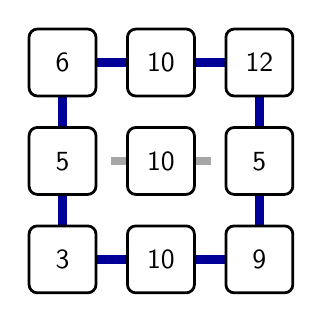
\begin{tikzpicture}[font=\sffamily,
    tile/.style={draw, rounded corners=3pt, fill=white, minimum size=0.85cm,
                 line width=1pt, inner sep=0pt},
    pipe/.style={line width=3pt, draw=blue!60!black},
    stub/.style={line width=3pt, draw=gray!70}]
  \def\s{1.25}
  % second test case of example 1: ring around the center
  \draw[pipe] (1*\s,-1*\s) -- (2*\s,-1*\s) -- (3*\s,-1*\s);
  \draw[pipe] (1*\s,-2*\s) -- (1*\s,-3*\s) -- (2*\s,-3*\s) -- (3*\s,-3*\s);
  \draw[pipe] (3*\s,-1*\s) -- (3*\s,-2*\s) -- (3*\s,-3*\s);
  \draw[pipe] (1*\s,-1*\s) -- (1*\s,-2*\s);
  % isolated center: openings to left/right that nobody answers
  \draw[stub] (2*\s,-2*\s) ++(-0.44,0) -- ++(-0.19,0);
  \draw[stub] (2*\s,-2*\s) ++( 0.44,0) -- ++( 0.19,0);
  \foreach \c/\r/\v in {1/1/6, 2/1/10, 3/1/12,
                        1/2/5, 2/2/10, 3/2/5,
                        1/3/3, 2/3/10, 3/3/9}
    \node[tile] at (\c*\s,-\r*\s) {\v};
\end{tikzpicture}
\end{document}
